% Load preamble
\RequirePackage[latest]{latexrelease}
\documentclass[a4paper,12pt]{article}
\usepackage[utf8]{inputenc}
\usepackage[T1]{fontenc}
\usepackage[a4paper]{geometry}
\usepackage{amsmath}
\usepackage{amssymb}
\usepackage{graphicx}
\usepackage{rotating}
\usepackage{placeins}
\usepackage[slovak]{babel}
\usepackage{makeidx}
\usepackage[colorlinks=true,linkcolor=blue,urlcolor=black]{hyperref}
\usepackage{bookmark}
\usepackage{bm}
\usepackage{cleveref}
%\usepackage{tikz}
\usepackage{multicol}
\usepackage{wrapfig}
%\usepackage{booktab}
\usepackage{array}
\usepackage{siunitx}
\usepackage{lmodern}
\usepackage{ellipsis}
\usepackage{nicefrac}
%\usepackage{microtype}
%\usetikzlibrary{positioning}

\crefname{equation}{rovn.}{rovn.}
\Crefname{equation}{Rovn.}{Rovn.}
\crefname{figure}{obr.}{obr.}
\Crefname{figure}{Obr.}{Obr.}
\crefname{table}{tab.}{tab.}
\Crefname{table}{Tab.}{Tab.}
\newcommand{\crefrangeconjunction}{ - }
\renewcommand{\figurename}{Obr.}
\renewcommand{\tablename}{Tab.}
\newcommand{\overbar}[1]{\mkern 1.5mu\overline{\mkern-1.5mu#1\mkern-1.5mu}\mkern 1.5mu}
\newcommand{\overhat}[1]{\mkern 1.5mu\hat{\mkern-1.5mu#1\mkern-1.5mu}\mkern 1.5mu}
\newcommand{\abs}[1]{|#1|}
\newcommand{\lint}{\int\limits}
\newcommand{\lsum}{\sum\limits}

\usepackage{parskip}% http://ctan.org/pkg/parskip
\usepackage[dvipsnames]{xcolor}
\begin{document}
\begin{titlepage}


\begin{center}
	\vspace*{5.5cm}
	 \textbf{\Huge Manuál ku GUI}\\
	 \vspace*{1cm}
	 Príloha k predmetu Tímový projekt	 
	
\end{center}
	\vspace*{9.5cm}
	\textbf{Vypracovali:} \hspace*{0.5cm} Bc. Eva Štalmachová\\
	 \hspace*{3.2cm} Bc. Ján Urdianyk\\ 
	 \hspace*{3.2cm} Bc. Denis Vasko\\
	 \hspace*{3.2cm} Bc. Marek Trebuľa
\end{titlepage}

\tableofcontents{}
\newpage


\section{Úvod}
Úlohou tohto grafického užívateľského rozhrania (ďalej len GUI) je zobrazovať, animovať, simulovať a reprezentovať správanie sa kyvadla. Pričom GUI má umožniť používateľovi jednoduchú zmeny fyzikálnych vlastností kyvadla, zmeny stavových veličín kyvadla (výchylka, uhlová rýchlosť) a možnosť apikácie rôzneho riadenia. GUI teda umožňuje skúšať zmeny parametrov samotného kyvadla alebo kyvadla spolu s riadením. Dôsledky týchto zmien je možné okamžite sledovať a prípadne vyhodnocovať kvalitu riadenia. 

GUI by sa mohlo stať pomôckou pre študentov, ktorá pomôže študentom získať jasnejšiu predstavu o prejednávaných problémoch pri opise, a návrhu riadenia nelineárnych systémov.

\newpage
\section{Opis simulovaného príkladu}
Ako bolo spomenuté v úvode GUI je určené sa simuláciu a opis hmotného bodu na závese (kyvadla). Nasledovná rovnica opisuje systém kyvadla:
\begin{equation}
mL^2\frac{d^2\Theta (t)}{dt^2} + B\frac{d\Theta (t)}{dt} + mgL sin(\Theta (t)) = u
\label{eqn:kyveq}
\end{equation}
\begin{center}
	\textit{m} - hmotnosť kyvadla\\
	\textit{L} - dĺžka závesu\\
	\textit{B} - tlmenie\\
	\textit{g} - gravitačné zrýchlenie ($9.81 m/s^2$)\\
	$\Theta$ - výchylka kyvadla\\
	\textit{u} - akčný zásah
	
		\begin{figure}[h!]
		\centering
		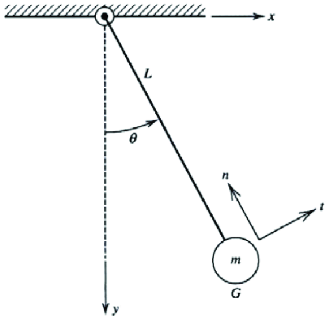
\includegraphics[width=0.8\linewidth]{pend}
		\caption{Náčrt kyvadla}
		\label{fig:pendulum}
	\end{figure}
	
\end{center}
 
\newpage
\section{Spustenie}
GUI bolo vytvorené v programe Matlab verzia 2018b. Spustenie je teda nutné vykonať priamo z Matlabu 2018b alebo \textbf{novšej} verzie. 
\subsection{Postup č. 1}
\begin{enumerate}
	\item Spustite program \textit{Matlab}.
	\item \textit{Current Folder} nastavte na priečinok, v ktorom sa nachádza súbor s názvom \textit{KyvGui.mlapp} (\cref{fig:spustenie}). 
	\begin{figure}[h!]
		\centering
		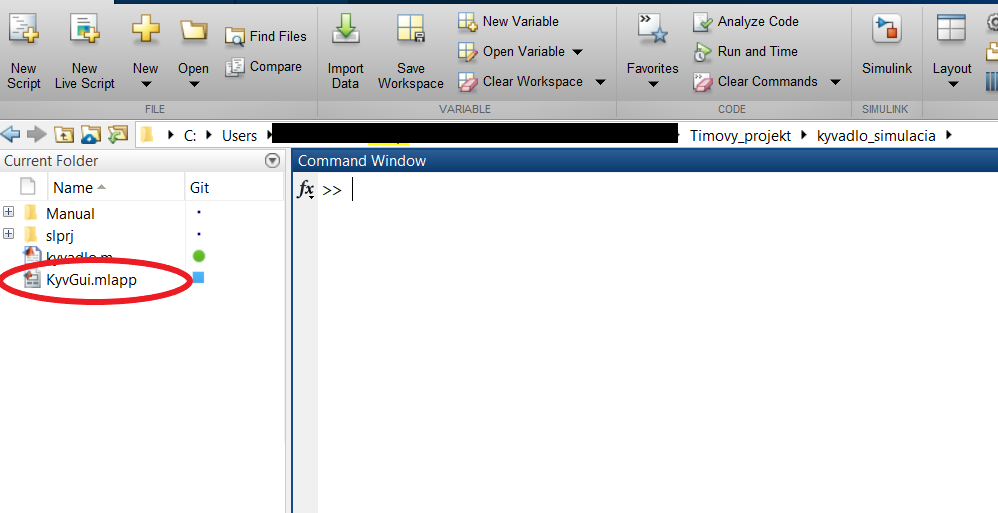
\includegraphics[width=0.9\linewidth]{spustenie1}
		\caption{Spustenie postup 1.}
		\label{fig:spustenie}
	\end{figure}
	\item Dvojklikom na \textit{KyvGui.mlapp} (zvýraznená položka na \cref{fig:spustenie}) spustíte GUI.
	
\end{enumerate}

\subsection{Postup č. 2 - editovanie}
\begin{enumerate}
	\item Spustite program \textit{Matlab}.
	\item \textit{Current Folder} nastavte na priečinok, v ktorom sa nachádza súbor s názvom \textit{KyvGui.mlapp} (\cref{fig:spustenie}).
	\item Do \textit{Command Window} napíšte príkaz \textit{>>appdesigner}. A stlačte Enter. Týmto príkazom ste spustili nástroj na tvorbu a \underline{editovanie} GUI (\cref{fig:spustenie2}).
	\begin{figure}[h!]
		\centering
		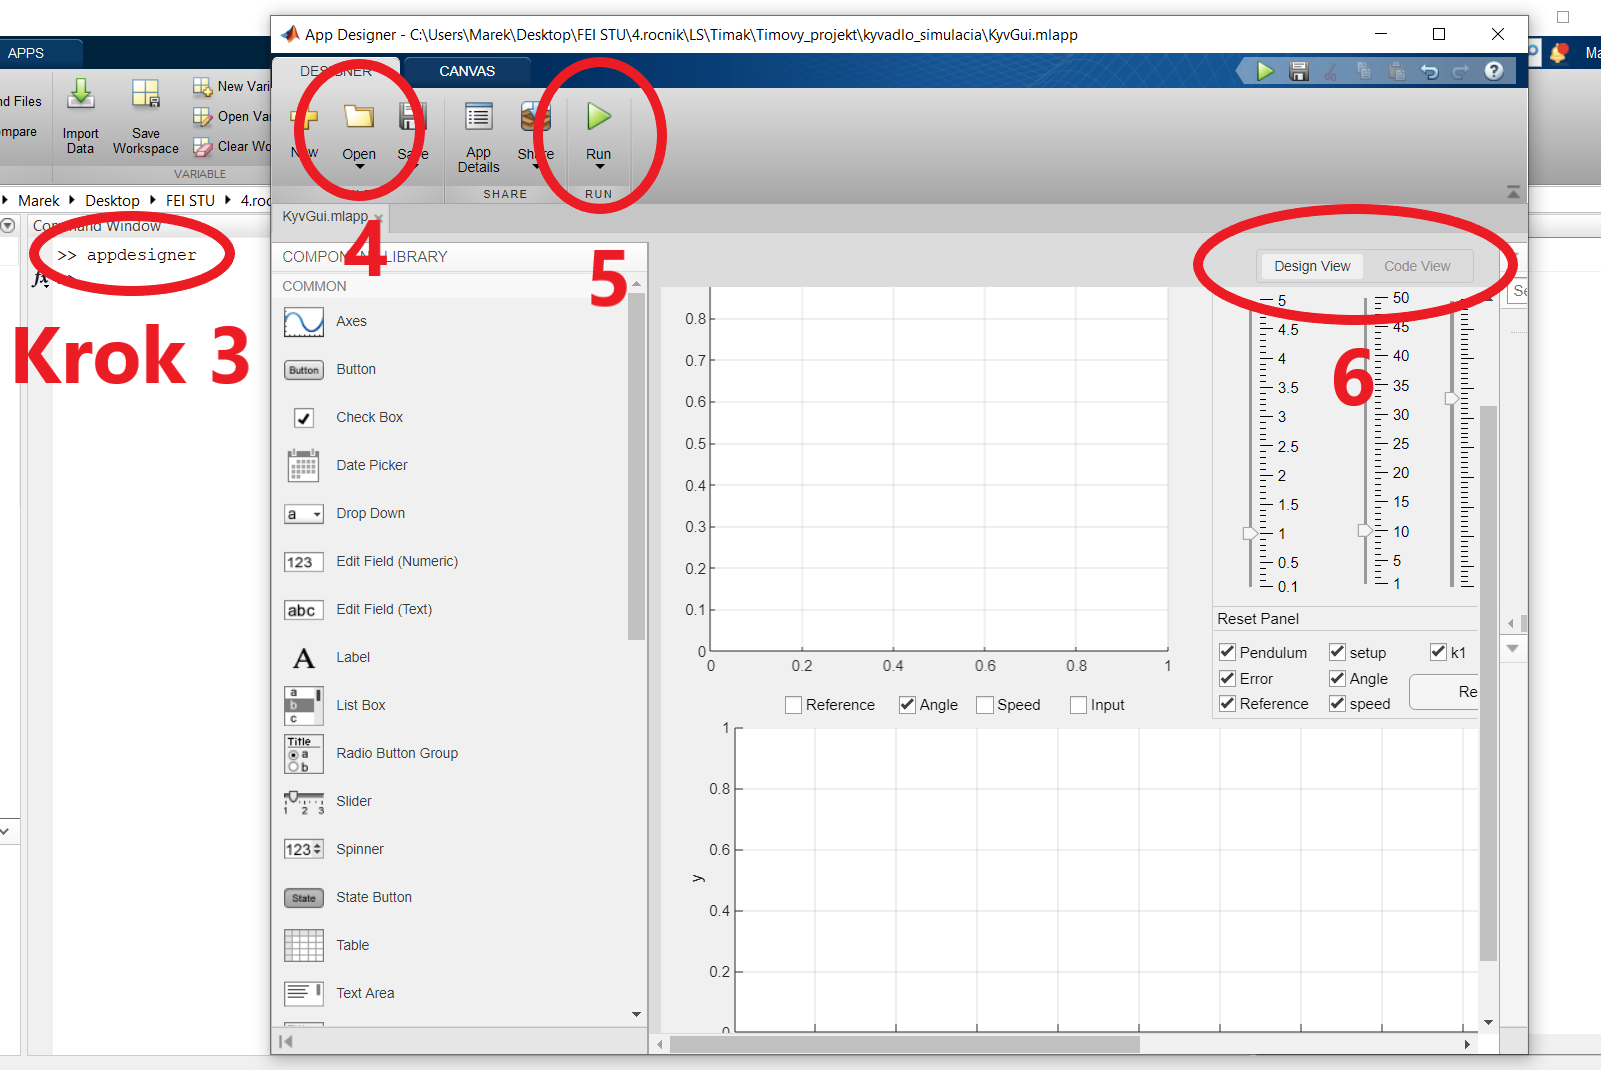
\includegraphics[width=0.9\linewidth]{spustenie2}
		\caption{Spustenie postup 2.}
		\label{fig:spustenie2}
	\end{figure}
    \item V hornej lište pomocou položky  \textit{Open} otvorte súbor \textit{KyvGui.mlapp}
    \item Potom pomocou položky  \textit{Run} spustíte GUI.
	\item Pomocou položky č. 6 môžete prepínať medzi zobrazením vzhľadu GUI a kódu GUI.
\end{enumerate}

\newpage
\section{Štruktúra GUI}
Po úspešnom spustení by ste mali vidieť nasledovné okno ako na \cref{fig:gui}.
	\begin{figure}[h!]
	\centering
	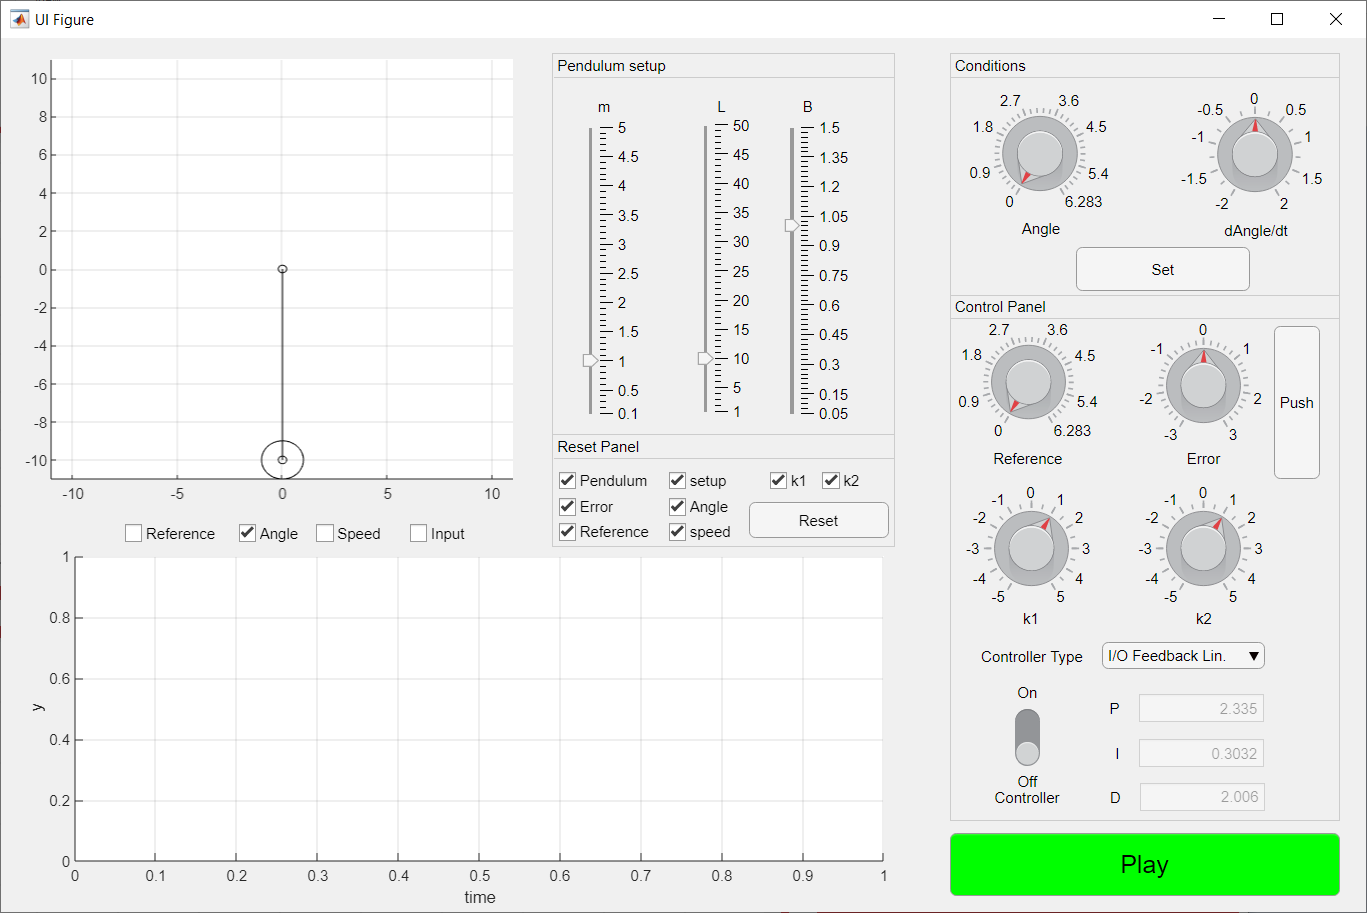
\includegraphics[width=0.9\linewidth]{gui}
	\caption{GUI}
	\label{fig:gui}
\end{figure}
Keďže GUI obsahuje relatívne veľa ovládacích prvkov, je rozčlenené na niekoľko panelov (skupín ovládacích prvkov, \cref{fig:structgui}). 

\subsection{Zoznam panelov}
\begin{enumerate}
	\item Okno animácie kyvadla.
	\item Okno priebehov veličín v čase.
	\item Panel výberu zobrazenia priebehov.
	\item Panel nastavenia fyzikálnych vlastností kyvadla.
	\item Panel resetovania nastavení.
	\item Panel nastavenia stavových veličín kyvadla.
	\item Panel riadenia.
	\item Tlačidlo \textbf{Play/Pause}.
\end{enumerate}

\makeatletter
\setlength{\@fptop}{0pt}
\makeatother

\begin{figure}[t!]
	\centering
	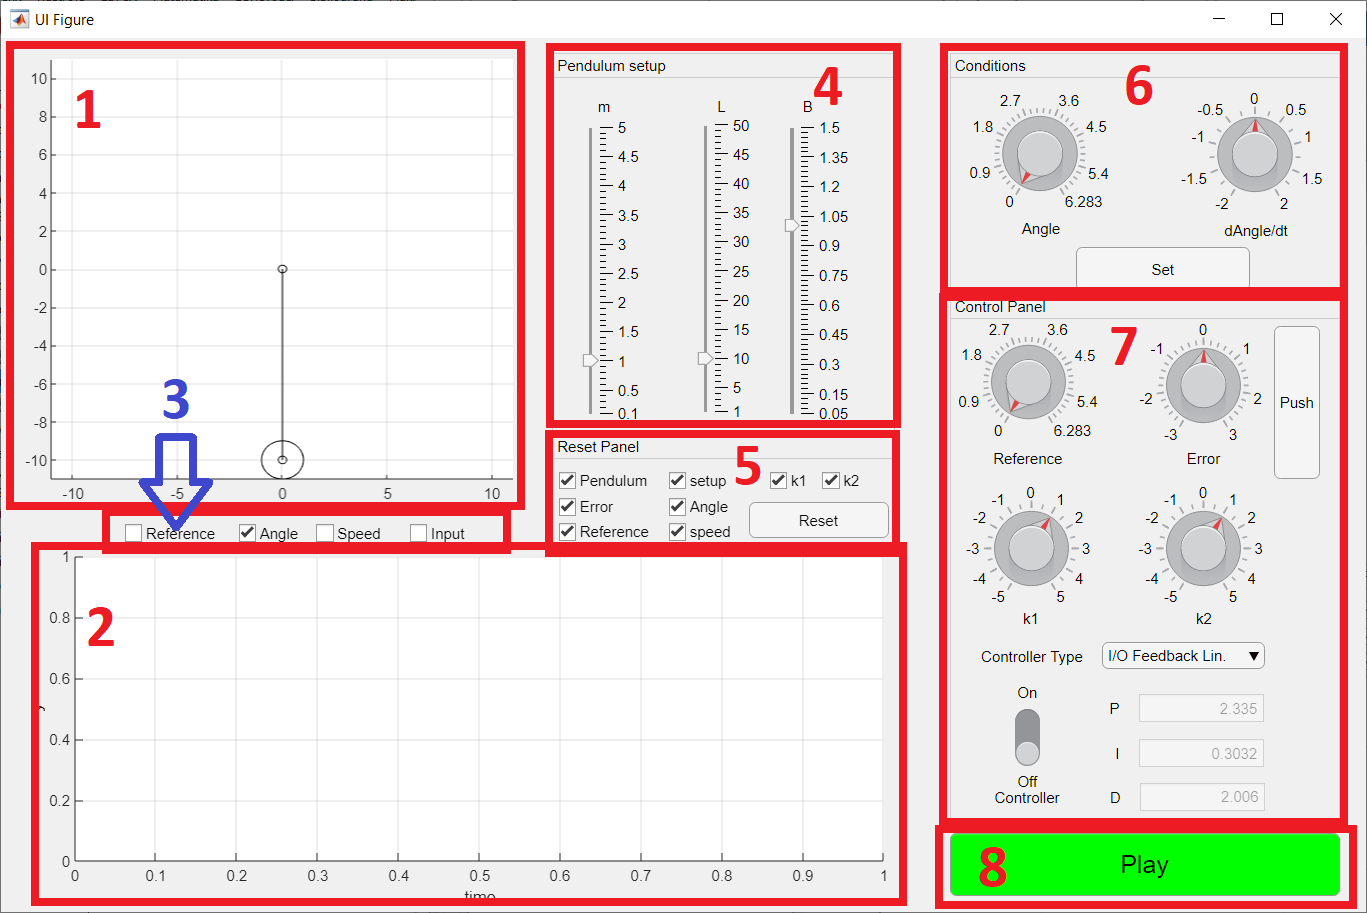
\includegraphics[width=0.9\linewidth]{structgui}
	\caption{Štrukturovanie GUI}
	\label{fig:structgui}
\end{figure}
 
 
\clearpage
\section{Ovládacie prvky}
\newpage
\section{Riadenie}

    
    

\end{document}